\chapter{Theoretical Foundations}\label{sec:theory}
\emph{Please note that all concepts introduced in Section~\ref{subsec:qubits} and Section~\ref{subsec:quantumlogicgates} can be found in any standard textbook on quantum information and will, therefore, not be referenced individually. Both of these sections are mainly based on the textbook by \citeA{nielsen2010quantum}.}
\section{Quantum bits}
\label{subsec:qubits}
\subsection{Single-qubit systems}
\label{subsubsec:qubits}

Classical computers manipulate bits, whereas quantum computer's most fundamental unit is called a \emph{quantum bit}, often abbreviated as \emph{qubit}. Instead of 0 and 1, qubit states are denoted \0 and \1 for reasons that will be outlined later.
%A non-probabilistic classical bit is a binary entity and can take either the value 0 or 1. Qubits are also binary entities but they can also be in a superposition of the two states. In contrast to classical bits, the two fundamental qubit states are denoted \0 and \1 for reasons outlined later.

A good example of a physical implementation of a qubit is the single electron of a hydrogen atom sketched in Fig.~\ref{img:qubitatom}. Usually, the electron is found in its ground state which one can define as the \0 state of the qubit. By using a laser pulse, the electron can be excited into the next higher valence shell which one can define as the \1 state of the qubit. After some time $t$ the electron will decohere to its ground state \0 which is called the \emph{longitudinal coherence} or \emph{amplitude damping time} and is an important parameter for measuring qubit lifetimes \cite{chuanglecturenotes}.

\begin{figure}[!ht]
       \centering
       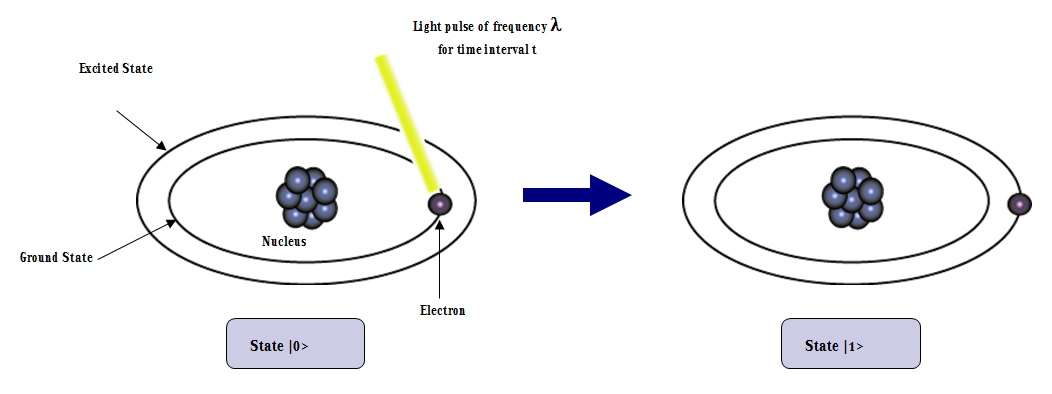
\includegraphics[scale=0.35]{img/qubitimplementation.jpeg}
       \caption[]{\label{img:qubitatom} A simple example of a physical qubit using the single valence electron of a hydrogen atom. Thereby, the electron's ground state can be defined as the \0 state of the qubit. By using a laser pulse, the electron can be excited into the next higher valence shell which can be defined as the qubit's \1 state. \textsuperscript{1}}
\end{figure}
\footnotetext[1]{Reprinted from RF Wireless World, n.d., Retrieved December 23, 2016, from \url{http://www.rfwireless-world.com/Terminology/Difference-between-Bit-and-Qubit.html}. Copyright 2012 by RF Wireless World.}

\pagebreak
A classical non-probabilistic bit can only take one of the two possible values at once. In contrast, qubits obey the laws of quantum mechanics, which gives rise to the important property that - besides being a definite \0 or \1 - they can also be in a superposition of the two states. Mathematically this is expressed as the linear combination of the states \0 and \1:
\begin{equation}
\label{equ: simplequbit}
\ket{\psi} = \alpha \ket{0} + \beta \ket{1}\, ,
\end{equation}
where $\alpha$ and $\beta$ are complex coefficients ($\alpha, \beta \in \mathbb{C}$) and are often referred to as amplitudes. Any amplitude $\eta$ can be further subdivided into a complex phase factor $e^{i\phi}$ and a non-negative real number $e$ such that
\begin{equation}
\label{equ: amplitude}
\eta = e^{i\phi}e\, .
\end{equation}
 
In Eq.~\ref{equ: simplequbit}, \0 is the Dirac notation for the qubit being in state 0 and can be represented as a two-dimensional vector in a complex two-dimensional vector space (called Hilbert space $\mathcal{H}_{2}$). First defined by \citeA{dirac1939new}, the object
\begin{equation}
\ket{\phi}\, ,
\end{equation}
is called a \emph{ket} and its Hermitian conjugate
\begin{equation}
\ket{\phi}^\dagger = \bra{\phi}\, ,
\end{equation}
is called a \emph{bra}. The Hermitian conjugate, denoted with a dagger ($\dagger$), of some e.g. two-dimensional column vector $c$ with complex entries $c_1$ and $c_2$:
\begin{equation}
c = \colvec{c_1\\c_2}\, ,
\end{equation}
is obtained by complex conjugating each entry and then transposing vector $c$:
\begin{equation}
c^\dagger = \colvec{c_1\\c_2}^\dagger = \begin{pmatrix}c_1^* & c_2^*\end{pmatrix}\, ,
\end{equation}
where complex conjugates are denoted with an asterisk ($*$). The Hermitian conjugate is defined for vectors as well as square matrices.

The inner product of a bra and a ket is called a \emph{bra-ket} and is written
\begin{equation}
\braket{\phi|\phi}
\end{equation}
Note that all later sections will make heavy use of this \emph{bra-ket notation}.

The quantum states \0 and \1 are called the computational basis states and they constitute an orthonormal basis of $\mathcal{H}_{2}$. When a qubit is expressed in terms of the two states \0 and \1 it is said to be in its \emph{standard basis}. For the sake of clarity, \0 and \1 can be represented as the 2-D vectors
\begin{equation}
\label{equ: 0and1kets}
\ket{0} \doteq  \colvec{1\\0} \quad \mathrm{and} \quad \ket{1} \doteq \colvec{0\\1} \, .
\end{equation}

Note that a ket and its vector representation are not the same object since a well-defined vector requires a basis whereas a ket does not demand specification of a basis. This thesis will make use of the $\doteq$ symbol when switching between the two different ways of representing a ket. Substituting the vectors from Eq.~\ref{equ: 0and1kets} into Eq.~\ref{equ: simplequbit} yields the vector representation of $\ket{\psi}$:
\begin{equation}
\label{equ: simplequbitvector}
\ket{\psi} \doteq \alpha \colvec{1\\0} + \beta \colvec{0\\1} = \colvec{\alpha\\\beta}\, .
\end{equation}

In the cases $\alpha = 1$ or $\beta = 1$ the qubit is not in a superposition but in the definite state \0 or \1 respectively. However, if for example $\alpha = \frac{1}{\sqrt{2}}$ and $\beta = \frac{i}{\sqrt{2}}$ the qubit is in a quantum superposition, impossible to achieve with a classical computer. This leads to another important qubit lifetime parameter - the \emph{transversal coherence} or \emph{phase damping time}. It is measured by preparing the equal superposition $\frac{\ket{0}+\ket{1}}{\sqrt{2}}$ and due to unavoidable interaction with the environment after some time $t$ the quantum behaviour will be lost, and the state will either be a definite \0 or \1 \cite{chuanglecturenotes}. The process of losing quantum behaviour is called \emph{decoherence}.

However, even though a qubit can be in a superposition of \0 and \1, when measured it will take the value \0 with a probability of
\begin{equation}
\label{equ:bornrule0}
\mathrm{Prob}(\ket{0}) = {|\alpha|}^{2}\, ,
\end{equation}
and \1 with a probability of 
\begin{equation}
\label{equ:bornrule1}
\mathrm{Prob}(\ket{1}) = {|\beta|}^{2}\, .
\end{equation}

The fact that the probability of measuring a particular state is equal the absolute value squared of the respective amplitude was first postulated by \cite{born1954statistical} and, thus, is called Born rule. Since the total probability of measuring any value has to be 1, the normalisation condition
\begin{equation}
\label{equ: normalization}
{|\alpha|}^{2} + {|\beta|}^{2} =  1\, ,
\end{equation}
must be satisfied. Therefore, a qubit is inherently probabilistic but when measured it collapses into a single classical bit (0 or 1). It follows that a measurement destroys information about the superposition of the qubit (the values of $\alpha$ and $\beta$). This constitutes one of the main difficulties when designing quantum algorithms since only limited information can be obtained about the final states of the qubits in the quantum computer.

Using spherical polar coordinates, a single qubit can be visualised on the so-called Bloch sphere by parameterising $\alpha$ and $\beta$ in Eq.~\ref{equ: simplequbit} as follows:
\begin{equation}
\label{equ: blochqubit}
\ket{\psi} = \cos\frac{\theta}{2} \ket{0} + e^{i \phi} \sin\frac{\theta}{2} \ket{1}\, .
\end{equation}
The Bloch sphere has a radius of 1 and is, therefore, a unit sphere. The \0 qubit state is defined to lie along the positive $\hat{z}$-axis and the \1 state is defined to lie along the negative $\hat{z}$-axis as labelled in Fig.~\ref{fig:blochsphere}. At this point, it is important to note that these two states are mutually orthogonal in $\mathcal{H}_{2}$ even though they are not orthogonal on the Bloch sphere. 

Qubit states on the Bloch equator such as the $\hat{x}$ and $\hat{y}$ coordinate axes represent equal superpositions where \0 and \1 both have measurement probabilities equal to $0.5$. The $\hat{x}$-axis for example represents the equal superposition $\ket{q} = \frac{1}{\sqrt{2}} \ket{0} + \frac{1}{\sqrt{2}} \ket{1}$. As illustrated in Fig.~\ref{fig:blochsphere} any arbitrary 2-D qubit state $\ket{\psi}$ can be decomposed into the polar angles $\theta$ and $\phi$ and visualised as a vector on the Bloch sphere. Such an object is called the Bloch vector of the qubit state $\ket{\psi}$. The Bloch sphere will be the main visualisation tool for qubit manipulations in this thesis.

\begin{figure}[!ht]
       \centering
       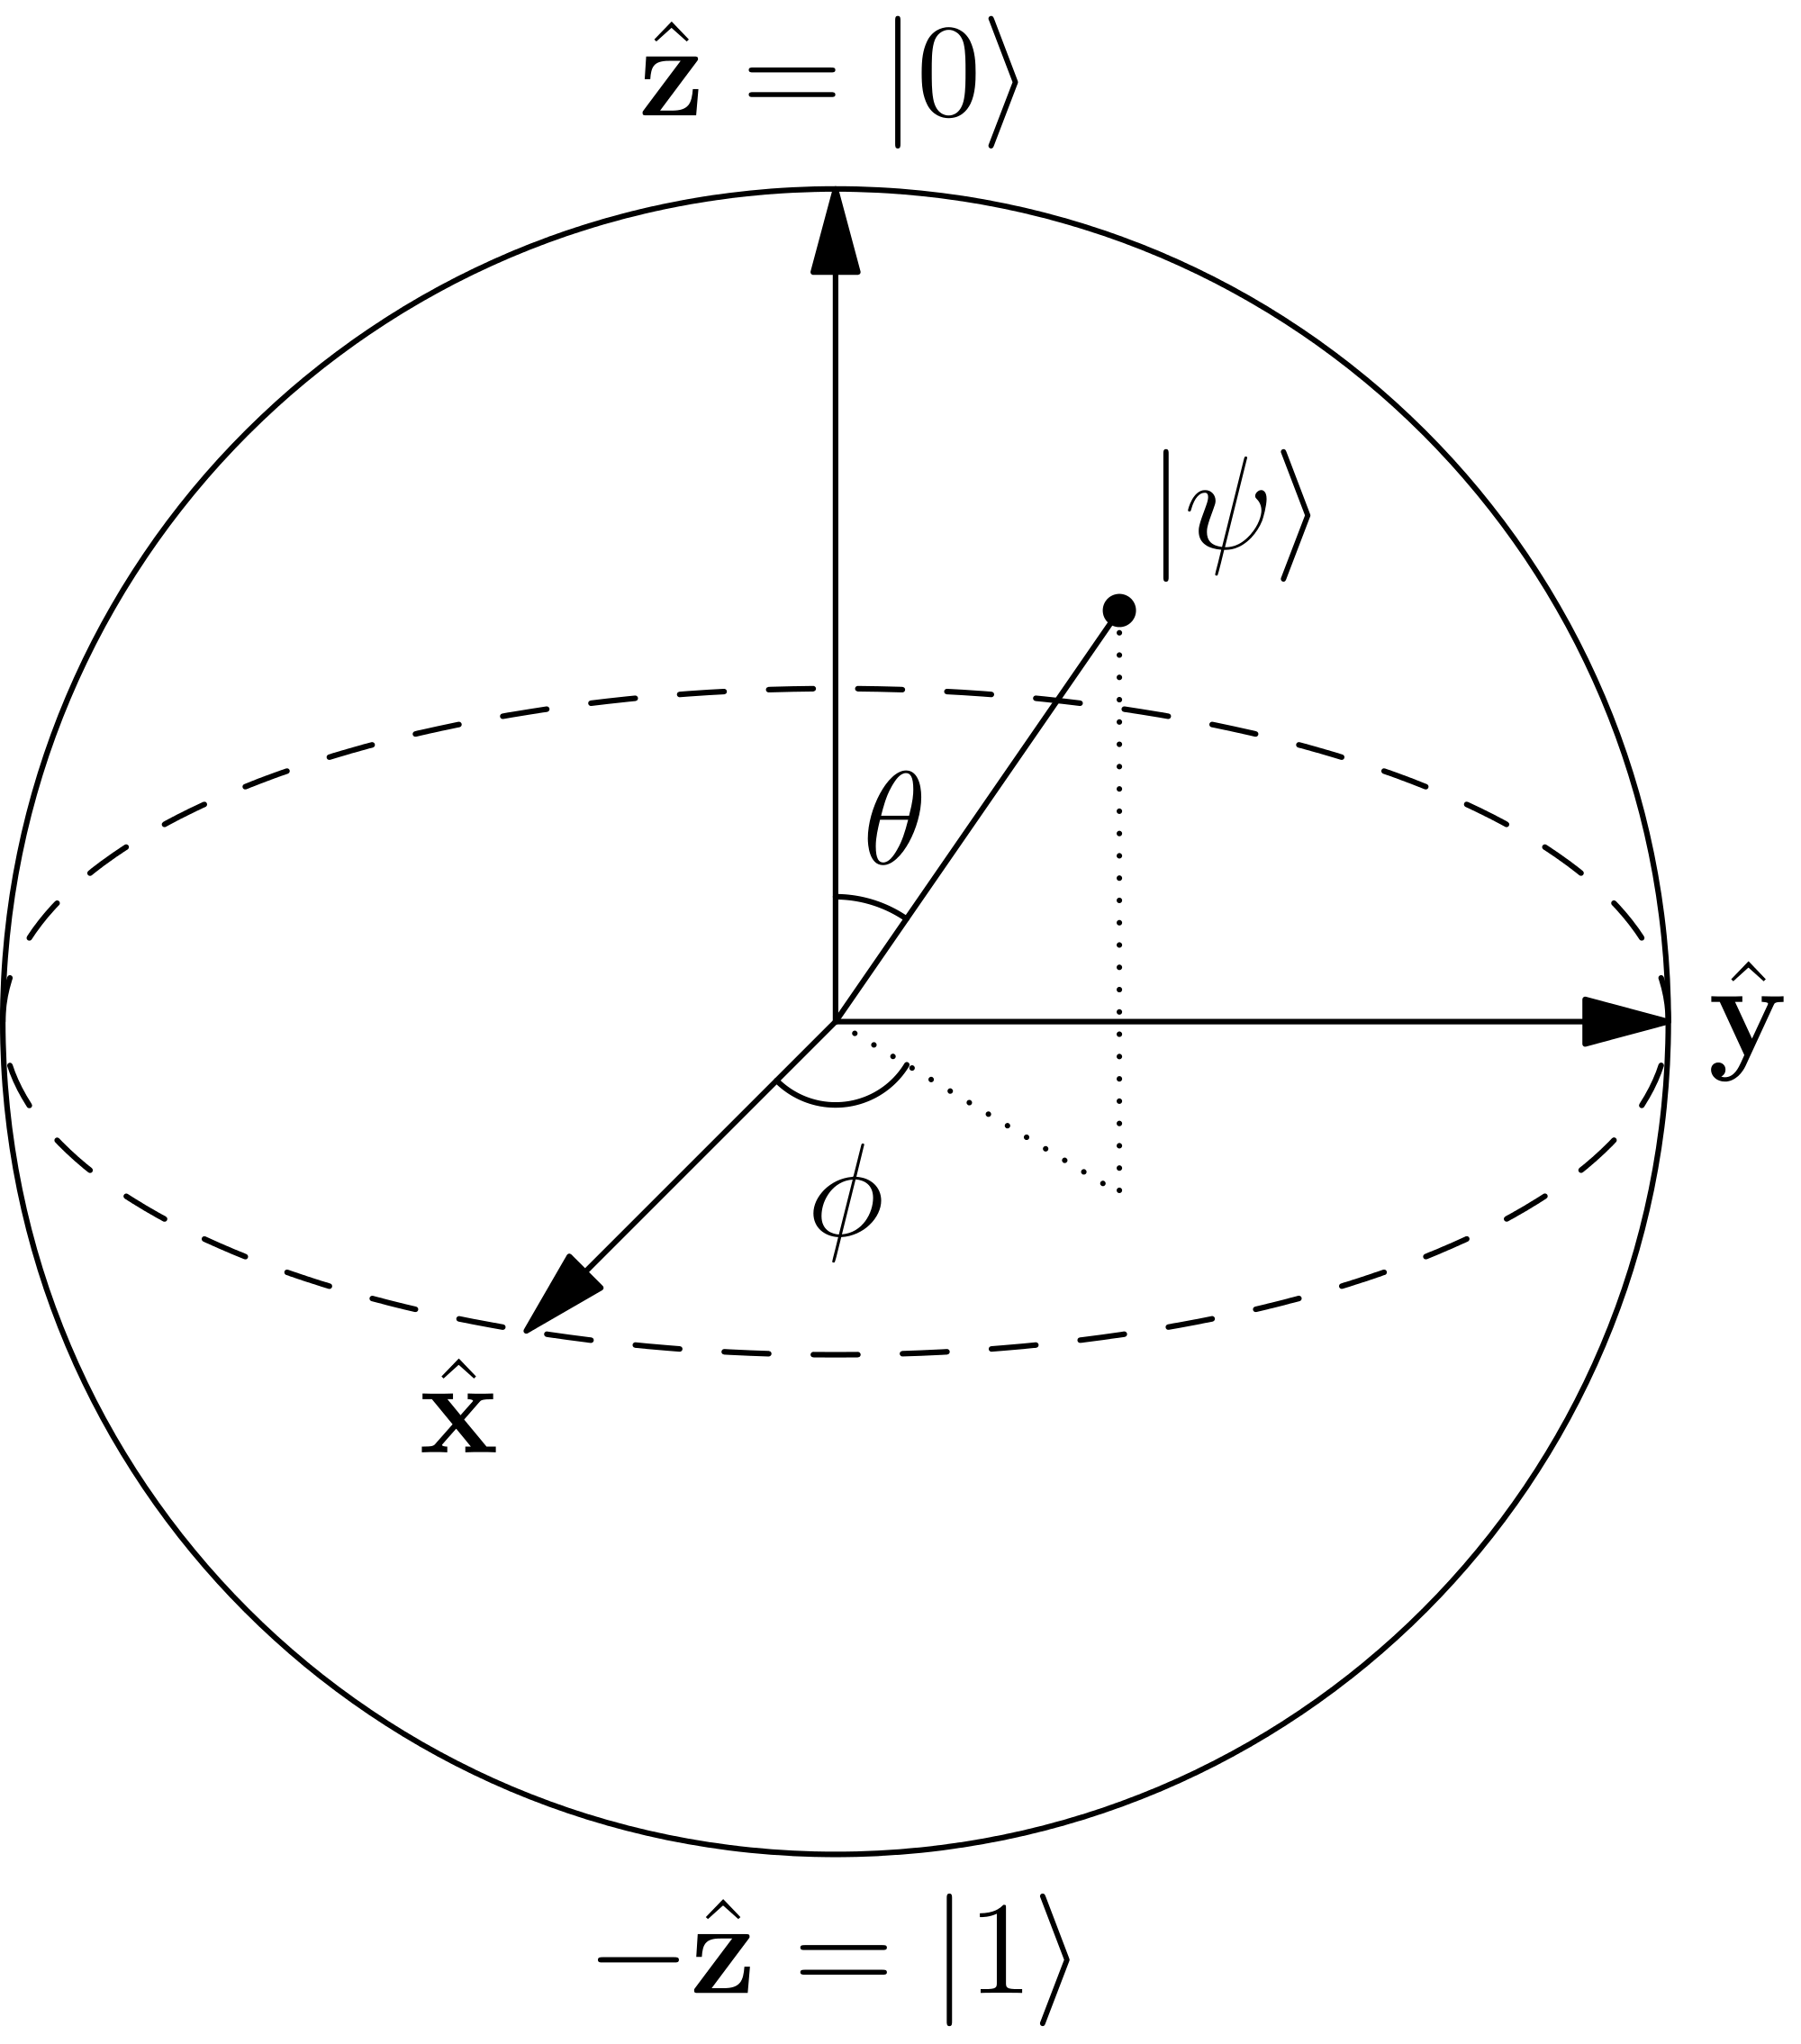
\includegraphics[scale=0.11]{img/blochsphere.png}
       \caption[]{\label{fig:blochsphere} An arbitrary single-qubit state $\ket{\psi} = \alpha \ket{0} + \beta \ket{1}$ can be visualised on the Bloch sphere by parameterising $\alpha = \cos\frac{\theta}{2}$ and $\beta = e^{i \phi} \sin\frac{\theta}{2}$ where $\theta$ is the polar and $\phi$ the azimuthal angle in spherical polar coordinates.\footnotemark[2]}
\end{figure}
\footnotetext[2]{Reprinted from Wikipedia, n.d., Retrieved September 7, 2016, from \url{https://en.wikipedia.org/wiki/Bloch_Sphere}. Copyright 2012 by Glosser.ca.}
\newpage

Similar to logic gates in a classical computer, a QC manipulates qubits, by means of quantum logic gates which will be introduced in detail in Section~\ref{subsec:quantumlogicgates}. Generally, an arbitrary quantum logic gate $U$ acting on a single qubit state is a unitary transformation which can be represented as a $2\times2$ matrix:
\begin{equation}
\label{equ:generalquantumgate}
U \doteq \begin{pmatrix}
 a & b \\ 
 c & d
 \end{pmatrix}\, ,
\end{equation}
whose action on $\ket{\psi}$ is defined as:
\begin{equation}
\label{equ:unitarytransformation}
U \ket{\psi} \doteq \begin{pmatrix}
 a & b \\ 
 c & d
 \end{pmatrix} \colvec{\alpha\\\beta} = \colvec{a\alpha+b\beta\\c\alpha+d\beta}\, .
\end{equation}

The matrix $U$ must be unitary which means that its determinant must equal unity:
\begin{equation}
\label{equ:unitarydef1}
\mid \mathrm{det}(U) \mid = 1\, ,
\end{equation}
and its Hermitian conjugate $U^\dagger$ must be equal to its inverse:
\begin{equation}
\label{equ:unitarydef2}
UU^\dagger = U^\dagger U = \mathbb{1} = UU^{-1} = U^{-1}U\, .
\end{equation} 

All quantum logic gates must be unitary since this preserves the normalisation of the qubit state it is acting on. The set of all two-dimensional complex unitary matrices with determinant one is called the special unitary group $\mathrm{SU}(2)$ and all single-qubit quantum gates are therefore elements of $\mathrm{SU}(2)$. Furthermore, a gate set $G$ consisting of $m$ quantum-gates $g_1,g_2,...,g_m$ is called a \emph{universal quantum gate set} when it is a dense subset of $\mathrm{SU}(2)$ as defined in the red box below.
\vspace{0.5cm}
\begin{redbox}
\textbf{Definition: Dense Subset of $\mathbf{SU(2)}$}\\
\newline
The gate set $G$ is a dense subset of $\mathrm{SU}(2)$ when given any quantum gate $W \in \mathrm{SU}(2)$ and any accuracy $\epsilon > 0$ there exists a product $J$ of gates from $G$ which is an $\epsilon$-approximation to $W$ \cite{dawson2005solovay}.
\end{redbox}
%\pagebreak
\subsection{Multi-qubit systems}
\label{subsec:multiqubitsystems}

A classical computer with one bit of memory is not particularly useful, and equally, a QC with one qubit is rather useless. To be able to perform large and complicated computations many individual qubits need to be combined to create a large QC. When moving from single to multi-qubit systems a new mathematical tool, the so-called tensor product (symbol $\otimes$), is needed. A tensor product of two qubits is written as
\begin{equation}
\label{equ:tensor}
\ket{\psi_1} \otimes \ket{\psi_2} = \ket{\psi_1}\ket{\psi_2} = \ket{\psi_1\psi_2}\, ,
\end{equation}
where the two last expressions omit the $\otimes$ symbol and are shorthand for a tensor product between two qubits.

A \emph{quantum register} of size $j$ is an alternative way of referring to a tensor product of $j$ qubits. For example, the state in Eq.~\ref{equ:tensor} is a quantum register consisting of two qubits. In QML algorithms, large quantum states are usually subdivided into several quantum registers fulfilling different purposes e.g. storing data or class labels. Consider, for example, a quantum state $\ket{\Phi}$ that is subdivided into two different quantum registers, a data ($d$) register with $n$ qubits and a class ($c$) register with two qubits. The state $\ket{\Phi}$ is then written
\begin{equation}
\label{equ:quantumregister}
\ket{\Phi} = \ket{d;c} = \ket{d_1,...,d_n;c_1,c_2}\, ,
\end{equation}
where semicolons are used to separate quantum registers.

In the vector representation a tensor product of two \0 kets (\textcolor{red}{red} and \textcolor{emerald}{green}) is defined as:
\begin{equation}
\label{equ:tensor2qubits}
\ket{\textcolor{red}{0}\textcolor{emerald}{0}} = \textcolor{red}{\ket{0}} \otimes \textcolor{emerald}{\ket{0}} \doteq \textcolor{red}{\colvec{1\\0}} \otimes \textcolor{emerald}{\colvec{1\\0}} = \colvec{\textcolor{red}{1}*\textcolor{emerald}{\colvec{1\\0}}\\\textcolor{red}{0}*\textcolor{emerald}{\colvec{1\\0}}} = \colvec{1\\0\\0\\0}\, .
\end{equation}

The last expression in Eq.~\ref{equ:tensor2qubits} shows that the two-qubit state $\ket{00}$ is no longer two but four-dimensional. Hence, it lives in a four-dimensional Hilbert space $\mathcal{H}_{4}$. A quantum gate acting on multiple qubits can therefore not have the same dimensions as a single-qubit gate (Eq.~\ref{equ:generalquantumgate}) which demands a new gate formalism for multi-qubit systems.

Consider aiming to apply an arbitrary single-qubit gate $U$ (Eq.~\ref{equ:generalquantumgate}) to the first qubit in the two-qubit state $\ket{00}$. The second qubit in the state $\ket{00}$ shall remain unchanged which, in other words, means applying the $2\times2$ identity matrix $\mathbb{1}$ to it. To perform these operations, one defines the tensor product of two single-qubit gates as
\begin{equation}
\label{equ:matrixtensorproduct}
\textcolor{red}{U} \otimes \textcolor{emerald}{\mathbb{1}} \doteq \textcolor{red}{\begin{pmatrix}
 a & b \\ 
 c & d
 \end{pmatrix}} \otimes \textcolor{emerald}{\begin{pmatrix}
 1 & 0 \\ 
 0 & 1
 \end{pmatrix}} = \begin{pmatrix}
 \textcolor{red}{a}*\textcolor{emerald}{\begin{pmatrix}
 1 & 0 \\ 
 0 & 1
 \end{pmatrix}} & \textcolor{red}{b}*\textcolor{emerald}{\begin{pmatrix}
 1 & 0 \\ 
 0 & 1
 \end{pmatrix}} \\ 
 \textcolor{red}{c}*\textcolor{emerald}{\begin{pmatrix}
 1 & 0 \\ 
 0 & 1
 \end{pmatrix}} & \textcolor{red}{d}*\textcolor{emerald}{\begin{pmatrix}
 1 & 0 \\ 
 0 & 1
 \end{pmatrix}}
 \end{pmatrix} = \begin{pmatrix}
 a & 0 & b & 0 \\ 
 0 & a & 0 & b \\ 
 c & 0 & d & 0 \\ 
 0 & c & 0 & d 
 \end{pmatrix}\, .
\end{equation}

Thus, the result of the tensor product $U \otimes \mathbb{1}$ can be represented as a unitary $4\times4$ matrix that can now be used to transform the $4\times1$ vector representing the $\ket{00}$ state in Eq.~\ref{equ:tensor2qubits}:
\begin{equation}
\label{equ:2qubitlineartransform1}
U \otimes \mathbb{1} \ket{00} \doteq \begin{pmatrix}
 a & 0 & b & 0 \\ 
 0 & a & 0 & b \\ 
 c & 0 & d & 0 \\ 
 0 & c & 0 & d 
 \end{pmatrix} \colvec{1\\0\\0\\0} = \colvec{a\\0\\c\\0}\, .
\end{equation}

One can also first perform the single qubit operations on the respective qubits, followed by the tensor product of the two resulting vectors:
\begin{equation}
\label{equ:2qubitlineartransform2}
(U \otimes \mathbb{1})(\ket{0} \otimes \ket{0})= U\ket{0} \otimes \mathbb{1}\ket{0} \doteq \begin{pmatrix}
 a & b \\ 
 c & d
 \end{pmatrix} \colvec{1\\0} \otimes \begin{pmatrix}
 1 & 0 \\ 
 0 & 1
 \end{pmatrix} \colvec{1\\0} = \colvec{a\\c} \otimes \colvec{1\\0} = \colvec{a\\0\\c\\0}\, .
\end{equation}

This formalism can be extended to any number of qubits, and the use of tensor products leads to an exponential increase in the dimensionality of the Hilbert space. Hence, $n$ qubits live in a $2^n$-dimensional Hilbert space ($\mathcal{H}_{2}^{\otimes n}$) and can store the content of $2^n$ classical bits. As an example, only 33 qubits can store the equivalent of $2^{33} = 8,589,934,592$ bits (= 1 gigabyte) which clearly bears the potential for enormous speedups in computations as will be demonstrated later.

When considering multi-qubit systems one will encounter quantum states that can or cannot be factorised. For example, consider reexpressing the last expression in Eq.~\ref{equ:2qubitlineartransform2} as
\begin{equation}
\label{equ:2qubitreexpressed}
\colvec{a\\0\\c\\0} = a\colvec{1\\0\\0\\0} + 0\colvec{0\\1\\0\\0} + c \colvec{0\\0\\1\\0} + 0\colvec{0\\0\\0\\1} \doteq  a\ket{00} + 0 \ket{01} + c \ket{10} + 0\ket{11}\, ,
\end{equation}
which can be factorised into the tensor product
\begin{equation}
\label{equ:2qubitfactorised}
a\ket{00} + c \ket{10} = (a\ket{0} + c \ket{1})\otimes \ket{0}\, .
\end{equation}

In contrast, consider one of the four famous Bell states:
\begin{equation}
\label{equ:2qubitnonfactorised}
\ket{\Psi^+} = \frac{\ket{01} + \ket{10}}{\sqrt{2}}\, .
\end{equation}
It is straightforward to verify that the two-qubit state $\ket{\Psi^+}$ cannot be factorised into a tensor product of two single-qubit states. Now imagine, that the two people Andile and Buhle are given two electrons prepared in the quantum state $\ket{\Psi^+}$. Andile keeps the first electron in the lab, and Buhle takes the second electron to her house. After some time $t$, Andile gets interested in measuring if his electron is in the $\ket{0}$ or $\ket{1}$ state and performs a measurement along the standard basis. By applying Born's rule to the quantum state $\ket{\Psi^+}$, Andile knows that he will measure his electron in either state \0 or \1 with equal probabilities of 0.5. Note that even though the exact state vector $\ket{\Psi^+}$ is known, the outcome of the measurement is still uncertain. By measuring his electron, he finds it to be in the $\ket{1}$ state. From Eq.~\ref{equ:2qubitnonfactorised} and knowing that measurement collapses a superposition, the post-measurement (PM) state $\ket{\Psi^+}_{PM}$ is
\begin{equation}
\label{equ:2qubitcollapsed}
\ket{\Psi^+}_{PM} = \ket{1_A0_B}\, ,
\end{equation}
where the subscripts indicate which electron belongs to Andile (A) and Buhle (B). Looking at this expression tells Andile that Buhle's electron must be in state $\ket{0}$ without having measured her electron! At her house, Buhle measures her electron one second after Andile has performed his measurement and indeed finds it to be in state $\ket{0}$. Note that the second electron was nowhere close to Andile and he was still able to determine its state by only measuring his electron. After repeating this experiment one thousand times, Andile and Buhle find perfect correlations in their results: whenever Andile measured his electron in state $\ket{0}$, Buhle found her electron in state $\ket{1}$ and vice versa.

Non-local correlations between qubit measurement outcomes is a peculiar quantum property of non-factorising quantum states and is called \emph{quantum entanglement}. It is an integral part of quantum computation and Section~\ref{subsubsubsec:cnotgate} will give a concrete example of how to create an entangled state in a QC.
%\pagebreak
\section{Quantum Logic Gates}
\label{subsec:quantumlogicgates}
Until this point, most introduced concepts came from the field of pure quantum theory. However, this section marks the important transition from quantum theory to the field of \emph{quantum information processing}. A classical computer processes information and performs computations by systematically manipulating bits through the application of logic gates e.g. NOT or XOR gates. Analogously, a quantum computer processes information and performs \emph{quantum computations} by manipulating qubits using \emph{quantum logic gates}, often just called \emph{quantum gates}. Usually, a sequence of such quantum gates is required to perform a certain task or solve a particular problem on a quantum computer. Such a sequence of quantum gates is called a \emph{quantum algorithm}. 

There are many different ways of realising a QC such as using trapped ions, photons or superconducting Josephson junctions, etc. \cite{clarke2008superconducting,haffner2008quantum,o2007optical}. Depending on the chosen substrate, different sets of quantum logic gates can be implemented and in order to run a quantum algorithm it has to be mapped to the available quantum hardware. Thus, quantum algorithms have to be translated (compiled) into a series of gates consisting only of quantum gates from the available universal gate set. This is referred to as \emph{quantum compiling}. 

The following subsections will introduce some major single and multi-qubit quantum logic gates that will be used extensively in the later sections of this thesis.
%In order to perform quantum computations, tools, analogous to the classical logic gates, are needed for qubit manipulation. 

\subsection{Single-qubit gates}
\label{subsubsec:singlequbitgates} 
%\subsubsection{Qubit flip (X) gate}
%\label{subsubsubsec:xgate}
%The quantum equivalent of the classical NOT logic gate is called X gate and is given by the 1\textsuperscript{st} Pauli matrix:
Quantum logic gates acting on single qubits can be represented as $2\times2$ unitary matrices (see Eq.~\ref{equ:generalquantumgate}) whose actions on a qubit can be visualised as rotations on the Bloch sphere. How a single-qubit quantum gate acts on a qubit, its properties and matrix representation will be illustrated using the example of the quantum equivalent of the classical NOT logic gate: the so-called X gate. The X gate can be represented by the $2\times2$ unitary matrix
\begin{equation}
X \doteq \begin{pmatrix}
 0 & 1 \\ 
 1 & 0
 \end{pmatrix}\, .
\end{equation}

The action of the X gate on the arbitrary qubit state $\ket{\psi}$ (Eq.~\ref{equ: simplequbitvector}) can be analysed using the gate's matrix and the qubit's vector representation. Applying some straightforward linear algebra yields
\begin{equation}
\label{equ:xverification1}
X \ket{\psi} = X (\alpha \ket{0} + \beta \ket{1}) \doteq \begin{pmatrix}
 0 & 1 \\ 
 1 & 0
 \end{pmatrix} \begin{pmatrix}
 \alpha  \\ 
 \beta
 \end{pmatrix} = \begin{pmatrix}
 \beta  \\ 
 \alpha
 \end{pmatrix} \doteq \beta \ket{0} + \alpha \ket{1}\, .
\end{equation}
Thus, applying the X gate to qubit state $\ket{\psi}$ swaps the amplitudes of the \0 and \1 states. More specifically, applying X to the \0 state results in the \1 state:
\begin{equation}
\label{equ:xverification2}
X \ket{0} \doteq \begin{pmatrix}
 0 & 1 \\ 
 1 & 0
 \end{pmatrix} \begin{pmatrix}
 1  \\ 
 0
 \end{pmatrix} = \begin{pmatrix}
 0  \\ 
 1 \end{pmatrix} \doteq  \ket{1}\, .
\end{equation}
In terms of the example with the valence electron of a hydrogen atom shown in Fig.~\ref{img:qubitatom} an X gate can be implemented by exciting the electron from the ground state $\ket{0}$ into the next higher electron valence shell, defined to be the $\ket{1}$ state, using a controlled laser pulse.
%consider the qubit initially being in state \0. Applying an X gate will flip the qubit into the \1 state which can be implemented in the lab by exciting the electron into the next highest electron valence shell using a controlled laser pulse.

The \0 state is recovered when applying X again to the \1 state:
\begin{equation}
\label{equ:xverification3}
X \ket{1} \doteq \begin{pmatrix}
 0 & 1 \\ 
 1 & 0
 \end{pmatrix} \begin{pmatrix}
 0  \\ 
 1
 \end{pmatrix} = \begin{pmatrix}
 1  \\ 
 0 \end{pmatrix} \doteq  \ket{0}\, .
\end{equation}

On the Bloch sphere, the X gate corresponds to an anti-clockwise $\pi$ rotation around the $\hat{x}$-axis as shown in Fig.~\ref{img:blochxgate}.

\begin{figure}[ht]
   \centering
   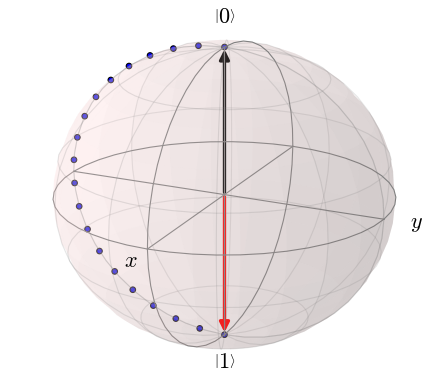
\includegraphics[width=0.75\textwidth]{img/blochxgate.png}
   \caption{Visualisation of the X gate action on the Bloch sphere. The figure shows the X gate transforming the \0 state (black $+\hat{z}$-axis) into the \1 state (red $-\hat{z}$-axis) by means of an anti-clockwise $\pi$ rotation around the $\hat{x}$-axis.}
   \label{img:blochxgate}
\end{figure}

From Eq.~\ref{equ:xverification1},~\ref{equ:xverification2} and~\ref{equ:xverification3} it follows that X is its own inverse as well as its own Hermitian conjugate:
\begin{align}
XX &= XX^\dagger = \mathbb{1}\, , \\
X &= X^{-1} = X^\dagger\, .
\end{align}

Based on the textbook by \citeA{nielsen2010quantum}, the action, circuit \& matrix representation and Bloch sphere visualisation for some of the most important single-qubit quantum logic gates are summarised in Table~\ref{tab:singlequbitgates}.

\begin{table}[H]
\caption{Table of some major single-qubit quantum logic gates.}\vspace{0.15em}
\label{tab:singlequbitgates}
\begin{tabular}{ C{0.3cm}  C{2cm}  C{1.5cm}  C{1.5cm} C{2.5cm} C{2cm} C{3.5cm}}\hline
Gate & Name & Circuit representation & Matrix & Description & Rotation & Bloch sphere \\ \midrule
$\mathbb{1}$ & Identity & 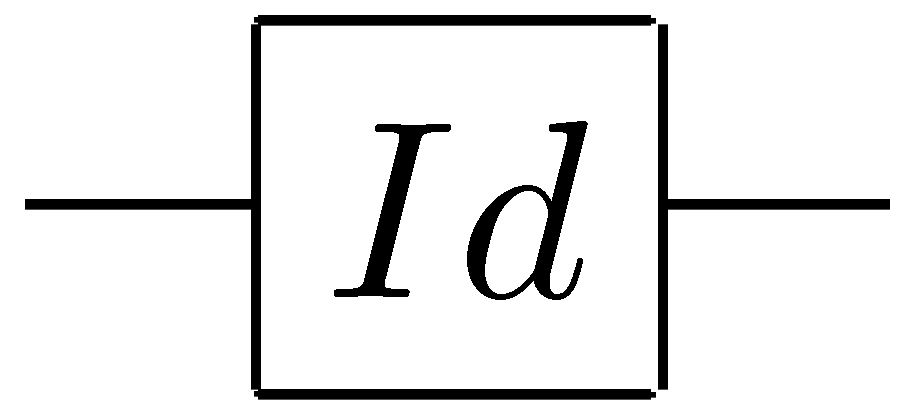
\includegraphics[width=0.1\textwidth]{img/identitycircuit.png} & $\begin{pmatrix}
 1 & 0 \\ 
 0 & 1
 \end{pmatrix}$ & Idle or waiting gate & - & - \\\midrule
X & Qubit flip & 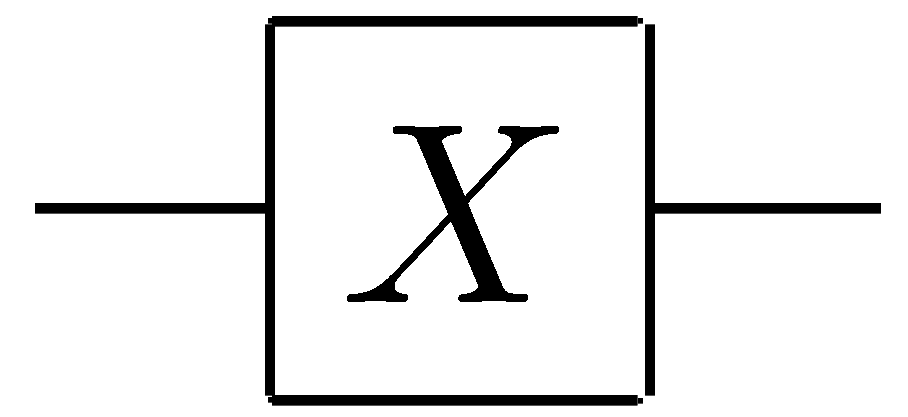
\includegraphics[width=0.1\textwidth]{img/xcircuit.png}  & $\begin{pmatrix}
 0 & 1 \\ 
 1 & 0
 \end{pmatrix}$ & Swaps amplitudes of \0 and \1 & $\pi$ rotation around $\hat{x}$ & 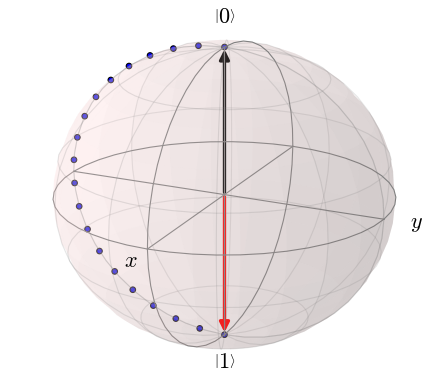
\includegraphics[width=0.2\textwidth]{img/blochxgate.png}\\\midrule
Y & Qubit \& phase flip & 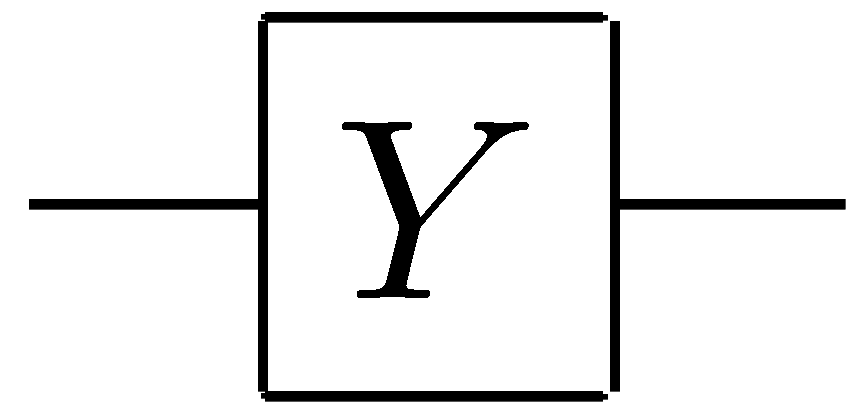
\includegraphics[width=0.1\textwidth]{img/ycircuit.png}  & $\begin{pmatrix}
 0 & -i \\ 
 i & 0
 \end{pmatrix}$ & Swaps amplitudes and introduces phase factor of $\pi$ (negative sign) to the \0 state & $\pi$ rotation around $\hat{y}$ &  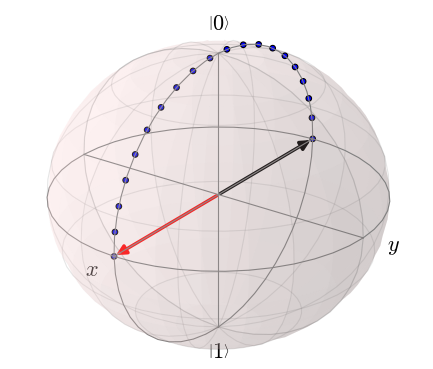
\includegraphics[width=0.2\textwidth]{img/blochygate.png}\\\midrule
Z & Phase flip & 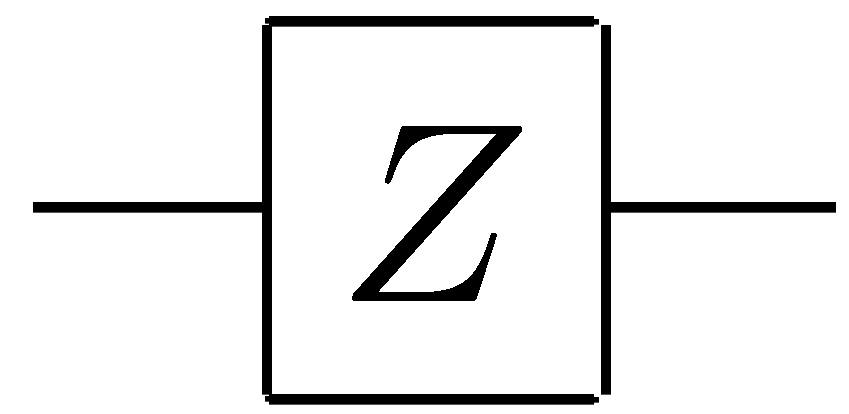
\includegraphics[width=0.1\textwidth]{img/zcircuit.png} & $\begin{pmatrix}
 1 & 0 \\ '
 0 & -1
 \end{pmatrix}$ & Introduces phase factor of $\pi$ (negative sign) to the \1 state & $\pi$ rotation around $\hat{z}$ & 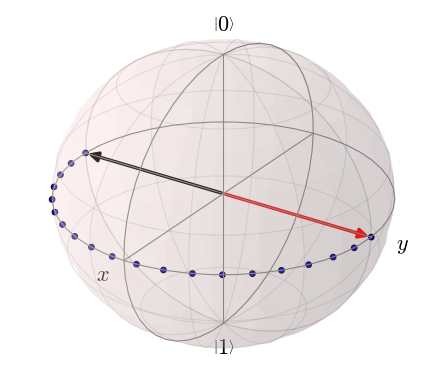
\includegraphics[width=0.2\textwidth]{img/blochzgate.png} \\\midrule 
H & Hadamard & 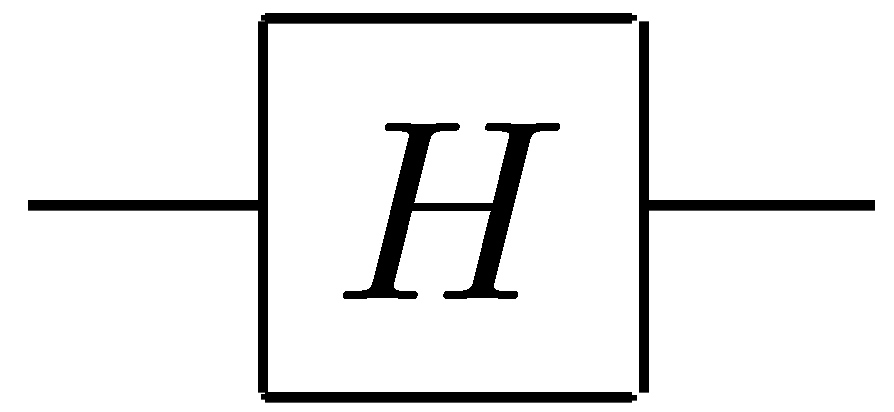
\includegraphics[width=0.1\textwidth]{img/hcircuit.png}  & $\begin{pmatrix}
 \frac{1}{\sqrt{2}} & \frac{1}{\sqrt{2}} \\ 
 \frac{1}{\sqrt{2}} & -\frac{1}{\sqrt{2}}
 \end{pmatrix}$ & Creates equal superposition & $\frac{\pi}{2}$ rotation around $\hat{y}$ and $\pi$ rotation around $\hat{x}$ & 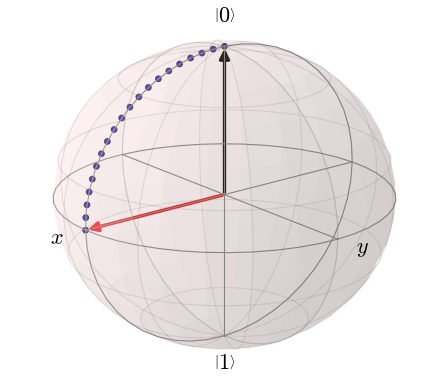
\includegraphics[width=0.2\textwidth]{img/blochhadamard.png}\\\midrule
S & $\frac{\pi}{2}$ rotation gate & 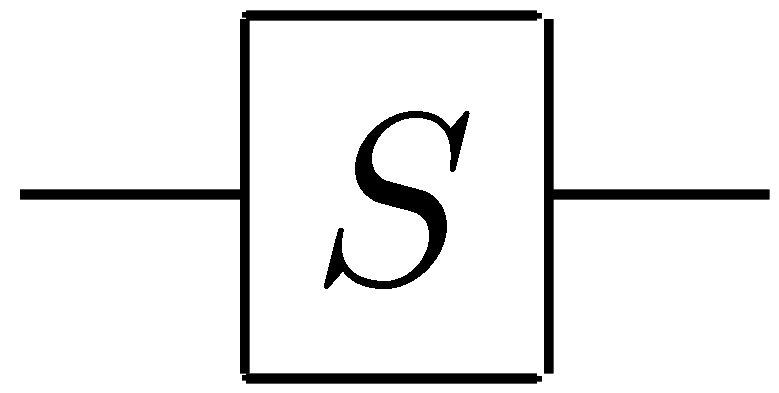
\includegraphics[width=0.1\textwidth]{img/scircuit.png} & $\begin{pmatrix}
 1 & 0 \\ 
 0 & i
 \end{pmatrix}$ & $\sqrt{Z}$ & $\frac{\pi}{2}$ rotation around $\hat{z}$ &  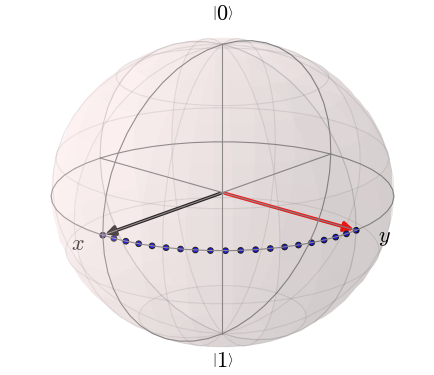
\includegraphics[width=0.2\textwidth]{img/blochsgate.png}\\\midrule
S$^\dagger$ & $-\frac{\pi}{2}$ rotation gate & 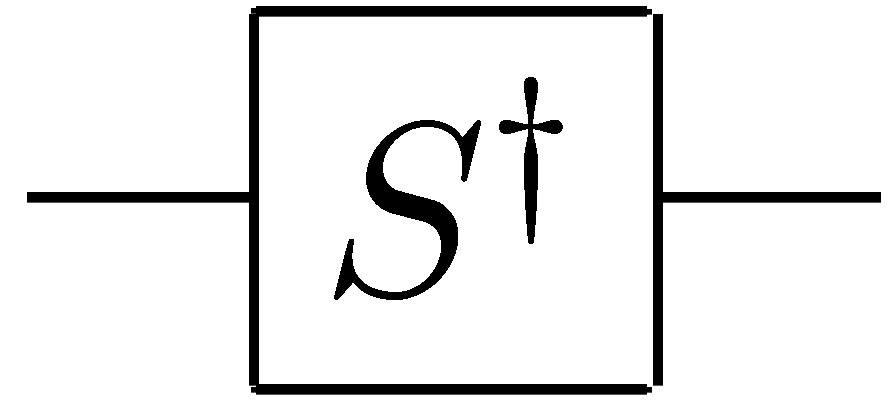
\includegraphics[width=0.1\textwidth]{img/sdcircuit.png} &  $\begin{pmatrix}
 1 & 0 \\ 
 0 & -i
 \end{pmatrix}$ & Hermitian conjugate of S & $-\frac{\pi}{2}$ rotation around $\hat{z}$ & \\\midrule
T & $\frac{\pi}{4}$ rotation gate & 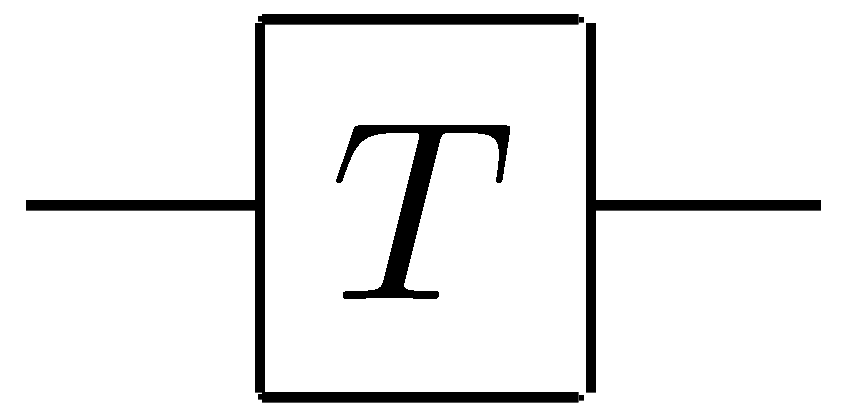
\includegraphics[width=0.1\textwidth]{img/tcircuit.png} & $\begin{pmatrix}
 1 & 0 \\ 
 0 & e^{\frac{i\pi}{4}}
 \end{pmatrix}$ & $\sqrt{S}$ & $\frac{\pi}{4}$ rotation around $\hat{z}$ & 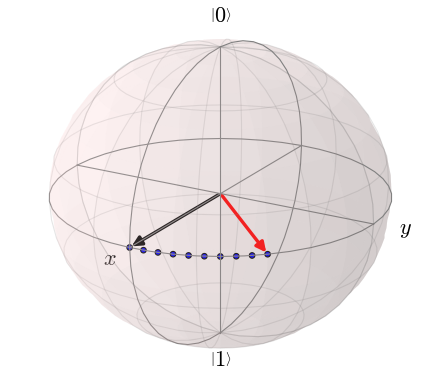
\includegraphics[width=0.2\textwidth]{img/blochtgate.png}\\\midrule
T$^\dagger$ & $-\frac{\pi}{4}$ rotation gate & 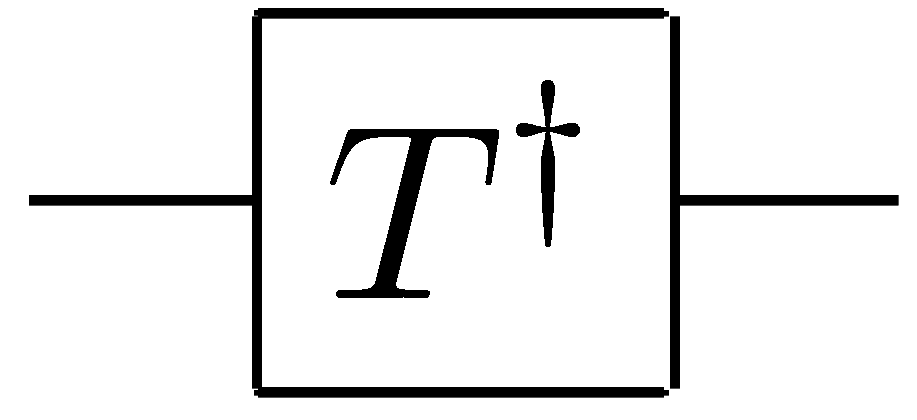
\includegraphics[width=0.1\textwidth]{img/tdcircuit.png} & $\begin{pmatrix}
 1 & 0 \\ 
 0 & e^{-\frac{i\pi}{4}}
 \end{pmatrix}$ & Hermitian conjugate of T & $-\frac{\pi}{4}$ rotation around $\hat{z}$ & \\\midrule
ZM & Z-basis measurement & 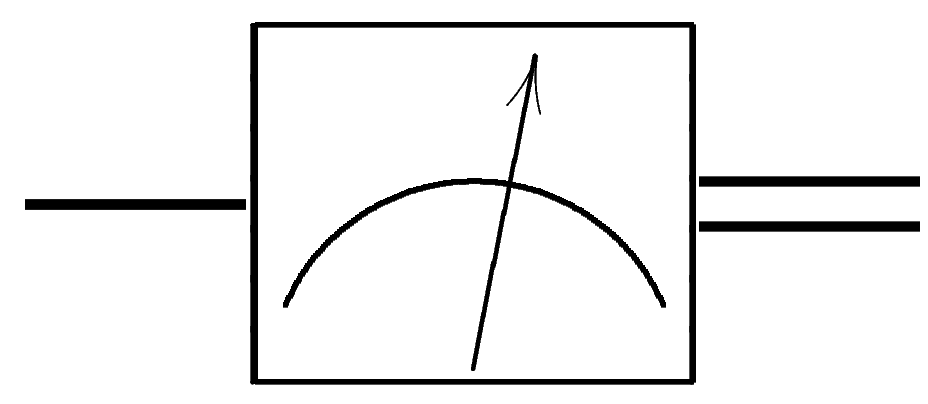
\includegraphics[width=0.1\textwidth]{img/measurecircuit.png} & - & Measurement in standard basis & Collapses the state & - \\
%\midrule
%BM & Bloch measurement & 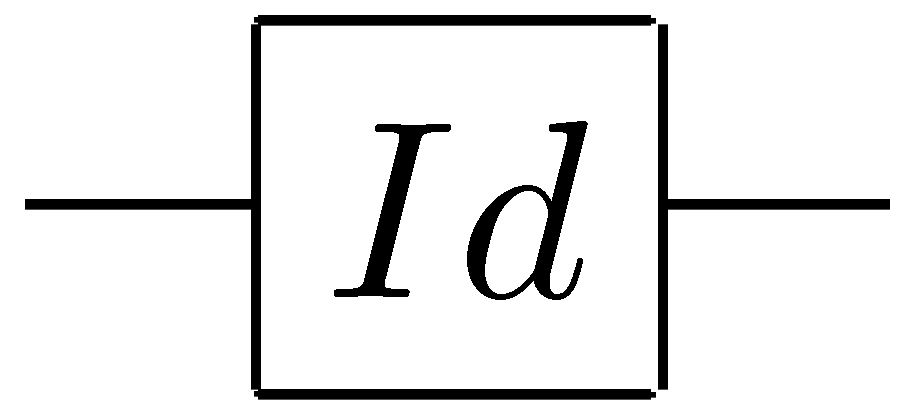
\includegraphics[width=0.1\textwidth]{img/identitycircuit.png} & - & Quantum state tomography & Collapses the state  & -\\
\end{tabular}
\end{table}


%%%%% SUBSECTION: MULTIPLE Q LOGIC GATES
\subsection{Multi-qubit gates}
\label{subsubsec:multiqubitgates}
\begin{table}[H]
\begin{center}
\begin{tabular}{l|lccc}\hline
Input & Output \\ \hline
00 & 00 \\
01 & 01 \\
10 & 11 \\
11 & 10 \\ \hline
\end{tabular}
\end{center}
\caption{Truth table for the CNOT quantum gate with the first qubit as control and the second qubit as target.}\vspace{1ex}
\label{tab:cnottruthtable}
\end{table}
%\subsubsection{Controlled-NOT gate}
%\label{subsubsubsec:cnotgate}
Multi-qubit quantum logic gates act on at least two qubits at the same time. Similar to single-qubit gates, an $n$-qubit quantum gate can be represented as a $2^n\times2^n$ unitary matrix. Since they involve multiple qubits, the Bloch sphere cannot longer be used to visualise their action. The two-qubit controlled NOT quantum gate will be used to demonstrate the properties, matrix representation and action of a two-qubit quantum gate. This can then easily be generalised to $n$-qubit quantum gates.

The controlled NOT or CNOT gate is given by the following $4\times4$ matrix:
\begin{equation}
\mathrm{CNOT} \doteq \begin{pmatrix}
 \mathbb{1} & 0 \\ 
 0 & X
 \end{pmatrix} = \begin{pmatrix}
 1 & 0 & 0 & 0 \\ 
 0 & 1 & 0 & 0 \\
 0 & 0 & 0 & 1 \\
 0 & 0 & 1 & 0 \\
 \end{pmatrix}\, .
\end{equation}

The CNOT gate takes two qubits, a control and a target qubit, as input. If and only if the control qubit is in the \1 state, the NOT (X) quantum gate is applied to the target qubit. In equations, the CNOT will always be followed by parentheses containing the control (c) qubit followed by the target (t) qubit: CNOT(c,t). The input-output relation, called truth table, for the CNOT gate is given in Table~\ref{tab:cnottruthtable} at the top of the page.

To demonstrate the usefulness of the CNOT gate consider starting with two unentangled qubits both in the \0 state,
\begin{equation}
\ket{\phi_0} = \ket{0} \otimes \ket{0} = \ket{00}\, .
\end{equation}
Applying the H gate onto the first qubit yields the following (still unentangled) state:
\begin{equation}
\ket{\phi_1} = (H \otimes \mathbb{1}) \ket{\phi_0} = (H \otimes \mathbb{1}) \ket{00} = \frac{1}{\sqrt{2}} \ket{00} + \frac{1}{\sqrt{2}} \ket{10}\, .
\end{equation}
Now consider applying the CNOT gate to the state $\ket{\phi_1}$ whereby the control qubit is coloured in \textcolor{red}{red} and the target qubit is coloured in \textcolor{emerald}{green}:

\begin{equation}
\label{equ:cnotexamples}
CNOT(\textcolor{red}{0},\textcolor{emerald}{1}) (\frac{1}{\sqrt{2}} \ket{\textcolor{red}{0}\textcolor{emerald}{0}} + \frac{1}{\sqrt{2}} \ket{\textcolor{red}{1}\textcolor{emerald}{0}}) = \frac{1}{\sqrt{2}} \ket{\textcolor{red}{0}\textcolor{emerald}{0}} + \frac{1}{\sqrt{2}} (\textcolor{red}{\mathbb{1}} \otimes \textcolor{emerald}{X}) \ket{\textcolor{red}{1}\textcolor{emerald}{0}} = \frac{1}{\sqrt{2}} \ket{\textcolor{red}{0}\textcolor{emerald}{0}} + \frac{1}{\sqrt{2}} \ket{\textcolor{red}{1}\textcolor{emerald}{1}}\, .
\end{equation}
The last expression in Eq.~\ref{equ:cnotexamples} is one of the famous Bell states which are a set of four maximally entangled quantum states. Another Bell state was used in the entanglement example in Section~\ref{subsec:multiqubitsystems}. Thus, this example demonstrates how the CNOT gate is crucial for the generation of entangled states since it applies the X gate to a target qubit depending on the state of a second control qubit.
%was used as an example (Eq.~\ref{equ:2qubitnonfactorised}) for entanglement in Section~\ref{subsec:multiqubitsystems} and it 

The three most important multi-qubit quantum gates CNOT, Toffoli and nCNOT are characterised in Table~\ref{tab:multiqubitgates}.

\begin{table}[H]
\caption{Table containing some major multi-qubit quantum logic gates where $c_j$ stands for the j\textsuperscript{th} control qubit and $\mathbb{1}_k$ for the $k\timesk$ identity matrix.}\vspace{1em}
\label{tab:multiqubitgates}
\begin{tabular}{ c  C{1.8cm}  C{2cm}  c C{3cm}}\hline
Gate & Name & Circuit representation & Matrix & Description \\ \midrule
CNOT & Controlled NOT & 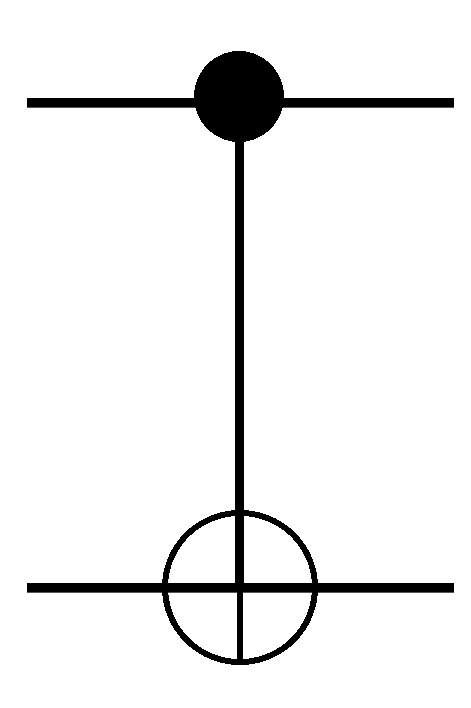
\includegraphics[width=0.1\textwidth]{img/cnotcircuit.png} & $\begin{pmatrix}
 \mathbb{1} & 0 \\ 
 0 & X
 \end{pmatrix} = \begin{pmatrix}
 1 & 0 & 0 & 0 \\ 
 0 & 1 & 0 & 0 \\
 0 & 0 & 0 & 1 \\
 0 & 0 & 1 & 0 \\
 \end{pmatrix}$ & CNOT($c_1$, target) \\\midrule
Toffoli & Controlled controlled NOT & 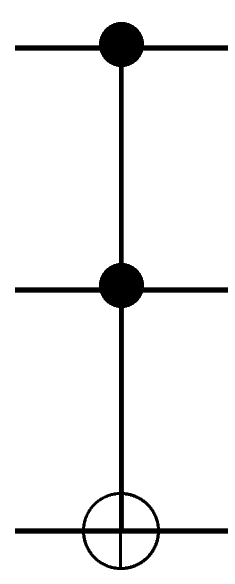
\includegraphics[width=0.1\textwidth]{img/ccnotcircuit.png}  & $\begin{pmatrix}
 \mathbb{1}_6 & 0 \\ 
 0 & X
 \end{pmatrix} = \begin{pmatrix}
 1 & 0 & 0 & 0 & 0 & 0 & 0 & 0 \\ 
 0 & 1 & 0 & 0 & 0 & 0 & 0 & 0 \\ 
 0 & 0 & 1 & 0 & 0 & 0 & 0 & 0 \\ 
 0 & 0 & 0 & 1 & 0 & 0 & 0 & 0 \\ 
 0 & 0 & 0 & 0 & 1 & 0 & 0 & 0 \\ 
 0 & 0 & 0 & 0 & 0 & 1 & 0 & 0 \\
 0 & 0 & 0 & 0 & 0 & 0 & 0 & 1 \\ 
 0 & 0 & 0 & 0 & 0 & 0 & 1 & 0 \\ 
 \end{pmatrix}$ & CCNOT($c_1$, $c_2$, target)\\\midrule
nCNOT & n-controlled NOT & -  & $\begin{pmatrix}
 \mathbb{1}_{2^n-2} & 0 \\ 
 0 & X
 \end{pmatrix}$ & nCNOT($c_1$,..,$c_n$, target) \\\midrule
\end{tabular}
\end{table}

%%%%% SECTION: MACHINE LEARNING

\section{Classical machine learning}
\label{subsec:classicalmachinelearning}

\emph{Machine learning} (ML), a subdiscipline of artificial intelligence, is trying to enable computers to learn from data without a human explicitly programming its actions. It can be subdivided into the three major fields \emph{supervised}, \emph{unsupervised} and \emph{reinforcement learning} \cite{schuld2015introduction}. Only supervised machine learning will be introduced because this thesis research exclusively focuses on supervised quantum machine learning algorithms. 

The main idea of supervised machine learning is to train an algorithm on a \emph{labelled} training dataset containing, for example, pictures of fruits with their corresponding names such that it can be used to label new pictures that are not part of the training dataset. Since the samples in the training dataset were labelled, the process is said to be supervised.

More formally, in supervised machine learning one is presented with pairs of input ($x$) and output ($o$) variables and the machine learning algorithm is supposed to learn the function $f$ that maps inputs to their respective outputs:
\begin{equation}
\label{equ:inputoutputML}
f(i) = o\, .
\end{equation}
Thereby, the algorithm should approximate the mapping function $f$ to such an extent that it can predict the output $o$ for new unknown input data $\tilde{x}$ \cite{bishop2006pattern}. The following section will introduce a well-known algorithm from the field of supervised ML: the classical $k$-nearest neighbour algorithm.

\newpage
\subsection{Classical $k$-nearest neighbour algorithm}
\label{subsubsec:knearestneighbour}

Understanding the quantum version of the distance weighted $k$-nearest neighbour (kNN) algorithm as proposed by \citeA{Schuld2014} requires prior knowledge of the classical version of the algorithm that will be introduced in this subsection.

Imagine working for a search engine company and you are given the task of classifying unknown pictures of fruits as either apples or bananas. To train your classification algorithm, you are given five different pictures of apples and five different pictures of bananas. This will be called the \emph{training data set} ${D}_{T}$. The pictures in ${D}_{T}$ may be taken from various angles, in varying light settings and include different coloured apples and bananas. Two examples of such images are shown in Fig.~\ref{img:appleandbanana}. 

\begin{figure}[H]
  \begin{minipage}[t]{0.48\textwidth}
    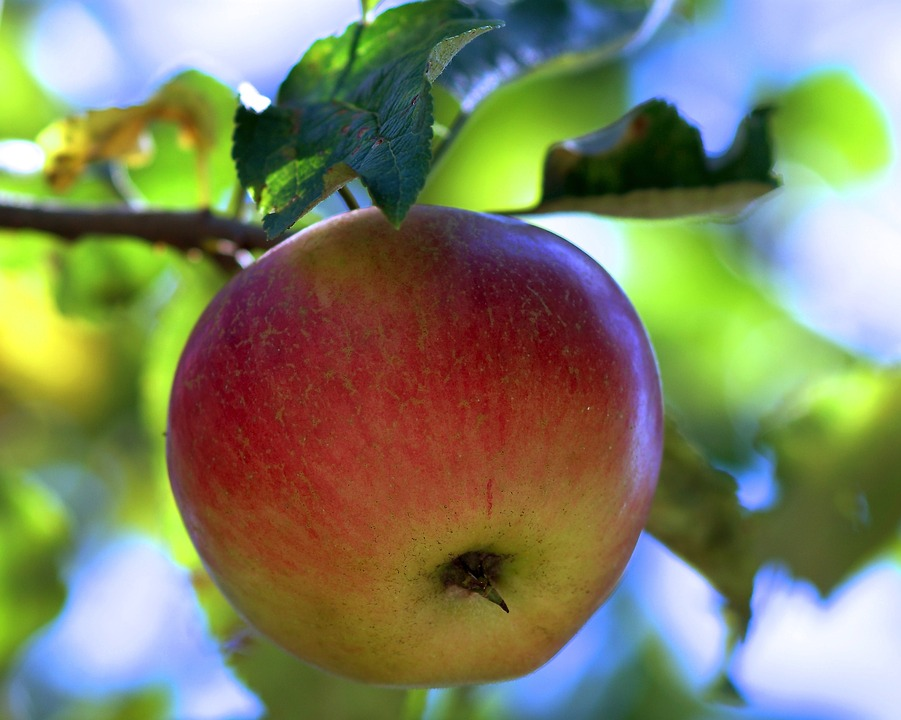
\includegraphics[width = \textwidth]{img/apple.jpg}
  \end{minipage}
  \hfill
  \begin{minipage}[t]{0.48\textwidth}
    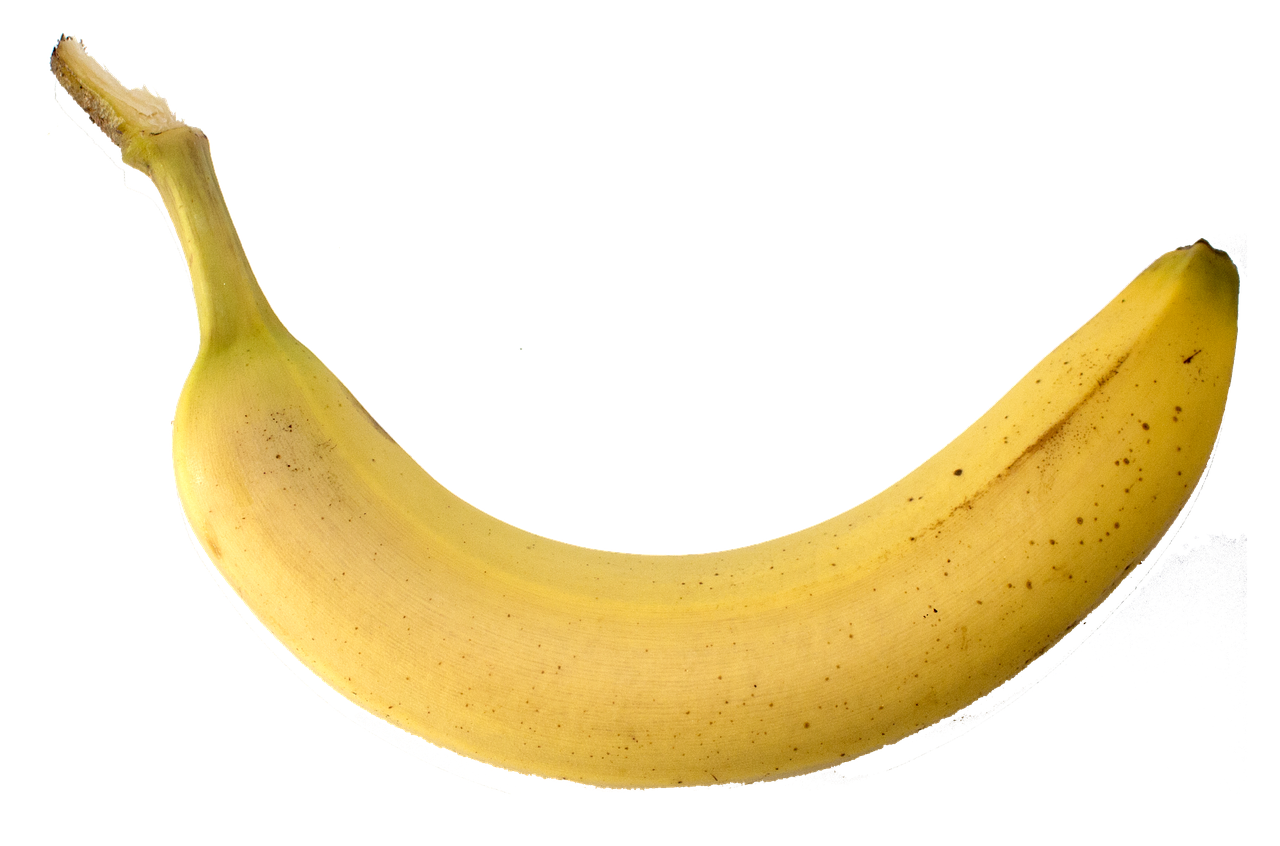
\includegraphics[width = \textwidth]{img/banana.png}
  \end{minipage}
  \caption[]{Example pictures of apple and banana from training data set ${D}_{T}$.\footnotemark[3]}
  \label{img:appleandbanana}
\end{figure}

\footnotetext[3]{Reprinted from Pixabay, Retrieved December 24, 2016, from \url{https://pixabay.com/en/apple-red-fruit-frisch-vitamins-1632016/} and \url{https://pixabay.com/en/banana-fruit-yellow-1504956/}. Creative Commons Licence 2016 by Pixabay.}

Most of the time, using the full pixel representation of each picture for classification does not lead to optimal results. Therefore, the next step is to select a certain number of characteristic \emph{features} extracted from the pictures in the training set that can be used to differentiate apples from bananas. Such a feature might be the RGB value of the most frequent pixel colour since bananas and apples have different colour spectra. Using a measure of the curvature of the main object in the picture is another possibility since an apple is almost spherical whereas a banana looks more like a bend line.

By selecting and extracting features, the dimensionality of the training data set is drastically reduced from a few thousand pixels to a handful of features. The $m$ extracted features for the j\textsuperscript{th} picture are stored in the $m$-dimensional \emph{feature vector} $\vec{v}_{j}$. Mathematically, the training data set ${D}_{T}$ consists of ten feature vectors $\vec{v}_{0}, \vec{v}_{1},..,\vec{v}_{10}$ that are each assigned to either class $A$ (apple) or $B$ (banana). The training vectors are visualised as yellow and purple circles in Fig.~\ref{fig:knnconcept}.

Given a new picture of either a banana or an apple, you first extract the same $m$ features from it and store it in the input vector $\vec{x}$. From many algorithms, you decide to use the kNN algorithm since it is a non-parametric classifier meaning it makes no prior assumption about the class of the new picture. Given a new unclassified input vector $\vec{x}$ (red star in Fig.~\ref{fig:knnconcept}), the algorithm considers the $k$ nearest neighbours within the training set (using a predefined measure of distance) and classifies $\vec{x}$, based on a majority vote, as either $A$ or $B$. Thereby, $k$ is a positive integer, usually chosen to be small and its value determines the classification outcome. Namely, in the case $k = 3$ in Fig.~\ref{fig:knnconcept}, vector $\vec{x}$ will be classified as class B (purple) but in the case $k = 6$ it will be labelled class A (yellow).

\begin{figure}[H]
      \centering
       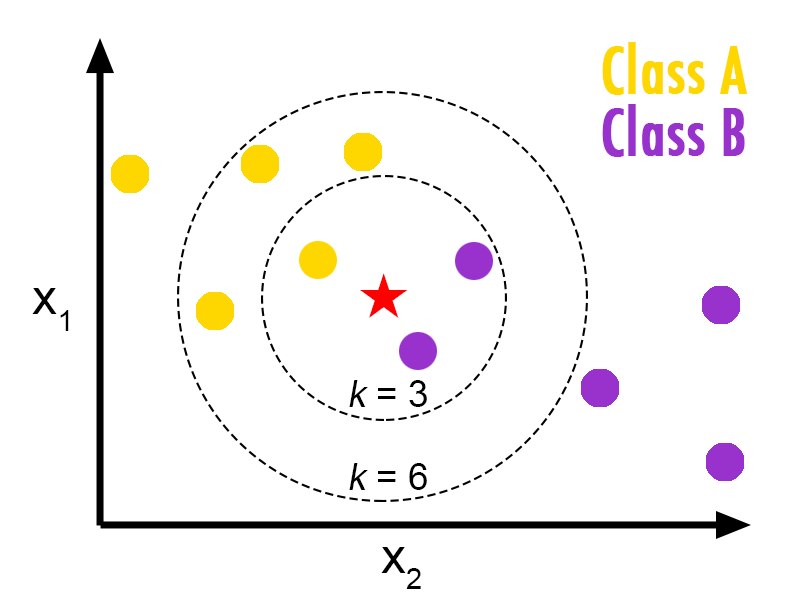
\includegraphics[scale=0.8]{img/knn-concept.png}
       \caption[]{\label{fig:knnconcept} Visualisation of a kNN classifier\footnotemark[4]}
\end{figure}

\footnotetext[4]{Reprinted from GitHub, Burton de Wilde, Retrieved September 13, 2016, from \url{http://bdewilde.github.io/blog/blogger/2012/10/26/classification-of-hand-written-digits-3/}. Copyright 2012 by Burton de Wilde.}

In the case of $k = 10$, $\vec{x}$ would simply be assigned to the class with the most members. In this case, the training vectors should be given distance-dependent weights (such as $\frac{1}{distance}$) to increase the influence of closer vectors over more distant ones.

\subsection{Algorithmic time complexity: Big-O notation}
\label{subsubsec:algcomplexity}

%\subsubsection{Big-O notation}
%\label{subsubsubsec:bigO}
In the fields of computer science and quantum information, the so-called \emph{Big-O notation}, first described by \citeA{bachmann1894analytische}, is often used to describe how the runtime of an algorithm depends on variables such as the desired accuracy, the number of input vectors or their size. Hence, this is a way of quantifying the \emph{algorithmic time complexity} of a quantum algorithm. In the later sections of this thesis, the Big-O notation will be used as a tool to quantify possible quantum speedups in kNN quantum machine learning algorithms.

\begin{redbox}
\textbf{Definition: Big-O $\mathcal{O}$}\\
\newline
For any monotonic functions $t(n)$ and $g(n)$ defined on a subset of the real numbers (${\rm I\!R}$), one says that $t(n) = \mathcal{O}(g(n))$ if and only if when there exists constants $c \geq 0$ and $n_0 \geq 0$ such that

\begin{equation}
\mid t(n) \mid \quad \leq \quad c\text{ }\mid g(n) \mid\, , \quad \text{for all } n \geq n_0\, .
\end{equation}
\end{redbox}
\begin{redbox}
\begin{figure}[H]
      \centering
       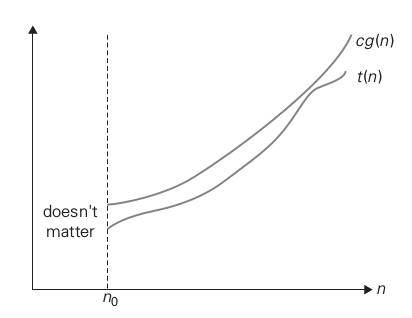
\includegraphics[scale=0.3]{img/asymptoticupperbound.png}
       \caption[]{\label{fig:upperasym} Visualisation of $c\text{ }g(n)$ being an upper asymptotic bound for the function $t(n)$\footnotemark[5]}
\end{figure}

\footnotetext[5]{Reprinted from Anany Levitin and Soumen Mukherjee. Introduction to the Design \& Analysis of Algorithms. Reading, MA: Addison-Wesley, 2003. Copyright 2012 by Levitin \& Mukherjee.}

This implies that the function $t(n)$ does not grow at a faster rate than $g(n)$, or in other words that some constant multiple of the function $g(n)$ is an upper asymptotic bound for the function $t(n)$, for all $n\rightarrow \infty$.
\end{redbox}

Fig.~\ref{fig:algcomplexities} provides a good visual comparison between common algorithmic complexity classes regarding their relation to the input size $n$. It can be seen that the best possible algorithmic time complexity is constant time, $\mathcal{O}(1)$, that is being independent of the size of the input data e.g. determining if a binary number is even or odd. An algorithm is still considered excellent if it runs in logarithmic time $\mathcal{O}(log(n))$. Linear search algorithms, for example, are linear in time expressed as $\mathcal{O}(n)$. More complex sort algorithms like "bubble sort" have a higher time complexity and often run in quadratic time ($\mathcal{O}(n^2)$). Furthermore, algorithms with complexity $\mathcal{O}(n^c)$ are said to run in polynomial time for some $c > 2$. If an algorithm has time complexity $\mathcal{O}((log(n))^c)$ for some $c \geq 1$ it is called polylogarithmic. The highest complexity classes are exponential $\mathcal{O}(c^n)$ with $c \geq 1$ and factorial time $\mathcal{O}(n!)$. 
%For example, solving the travelling salesman problem using brute-force search runs in factorial time.

\begin{figure}[H]
      \centering
       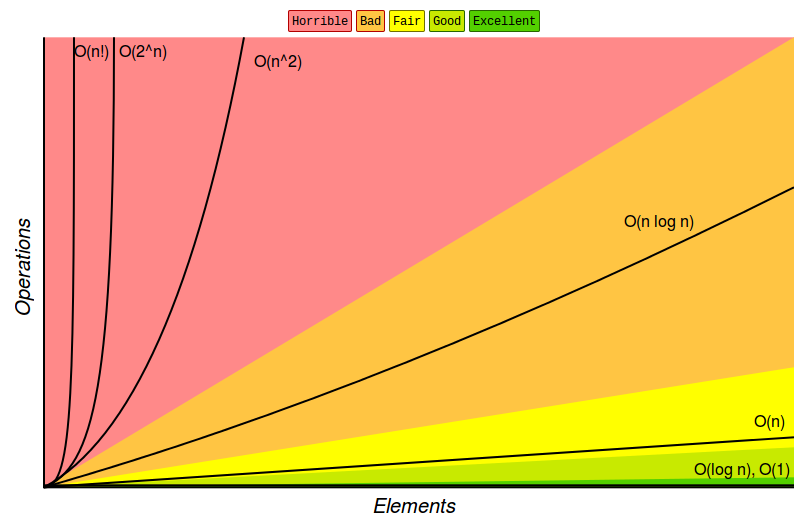
\includegraphics[scale=0.35]{img/bigocomplexity.png}
       \caption[]{\label{fig:algcomplexities} Overview of some major algorithmic complexity classes. In the figure, the number of operations (vertical axis) is plotted against the number of elements $n$ in the input data vector (horizontal axis). Based on colour coding defined on top of the table the following algorithmic time complexity classes are illustrated: constant time $\mathcal{O}(1)$, logarithmic time $\mathcal{O}(log(n))$, linear time $\mathcal{O}(n)$, linearithmic time $\mathcal{O}(n log(n))$, quadratic time $\mathcal{O}(n^2)$, exponential time $\mathcal{O}(2^n)$ and factorial time $\mathcal{O}(n!)$.\footnotemark[6]}
\end{figure}
\footnotetext[6]{Reprinted from Big-O Cheatsheet, Retrieved December 28, 2016, from \url{http://bigocheatsheet.com/}. Copyright 2016 by Big-O Cheatsheet.}

%TRANSITION TO NEXT SECTION NEEDED!